\documentclass[a4paper,10pt]{article}
\usepackage[utf8]{inputenc}
\usepackage[toc]{appendix}

\usepackage{csvsimple}
\usepackage{geometry}
\usepackage{graphicx}
\usepackage{hyperref}
\usepackage{setspace}
\usepackage{siunitx} % For rounding
\usepackage{titlesec}

\geometry{a4paper, margin=1in}
\doublespacing
\titleformat{\section}[block]{\normalfont\Large\bfseries}{\thesection}{1em}{}
\titleformat{\subsection}[block]{\normalfont\large\bfseries}{\thesubsection}{1em}{}
\titleformat{\subsubsection}[block]{\normalfont\normalsize\bfseries}{\thesubsubsection}{1em}{}

\begin{document}

\title{Carried away by Long Short-Term Memory: A Machine Learning Approach to Forecasting Carry Trade Returns}
\author{Anton Aleynikov \& Sergey Mirzoev}
\date{\today}
\maketitle

\begin{abstract}

\textbf{Carry trade}, a risky arbitrage strategy exploiting interest rate differentials between two currencies, challenges foreign exchange market efficiency. This research project builds upon the work of Wang et al. (2021) ~\cite{wang2021machine}, which employed long short-term memory (LSTM) networks to forecast carry trade returns. Using a data set spanning 1990 to 2017 for 11 countries, members of G10, the study found that LSTM models underperformed traditional threshold regression models based on simple economic fundamentals. Additionally, the research revealed a deterioration in excess carry trade returns after the 2007–2008 global financial crisis, suggesting a potential impact on the uncovered interest rate parity.
\end{abstract}

\section{Introduction}

% Brief overview of carry trade and its significance in the forex market.
% Introduction to the challenge of persistent excess carry trade returns and its implications for market efficiency.
% Reference to Wang et al. (2021) and their findings using LSTM networks.

Carry trade is a significant phenomenon in the forex market, affecting interest rate differentials, risk-return dynamics, market liquidity, and volume. However, the problem of excess carry trade returns poses a challenge to market efficiency. When carry trade returns exceed what would be expected based on interest rate differentials, it raises questions about the factors driving the extended abnormal returns and challenges the principles of the Efficient Market Hypothesis (\hyperref[appx:emh]{EMH}).

This concern calls for a closer examination of behavioural factors influencing trading decisions. To address this issue, this research builds on the work of Wang et al. (2021) ~\cite{wang2021machine} by using long short-term memory (\hyperref[appx:lstm]{LSTM}) networks to forecast carry trade returns, which is a novel approach compared to traditional models.

This study focuses on existing literature on carry trade and forecasting models, compares LSTM networks with linear and threshold regression models, and delves into the methodology, results, and implications for forex market efficiency and carry trade strategies.

The primary objective of this research is to improve our understanding of carry trade dynamics, with a focus on forecasting models. By comparing the LSTM approach with traditional models, we aim to evaluate the effectiveness of machine learning in predicting carry trade returns and contribute to the body of knowledge on this topic.

\section{Literature Review}
% Explore existing literature on carry trade and forecasting models.
% Discuss traditional models based on economic fundamentals.
% Introduce machine learning approaches, focusing on LSTM networks.

Carry trade, a risky arbitrage strategy based on interest rate differentials between currencies has been the subject of extensive research in financial economics. The returns from carry trades are intricately tied to changes in exchange rates and interest rate differentials across countries. Despite the challenges it poses to the Efficient Market Hypothesis (EMH), there is evidence suggesting that Uncovered Interest Parity (UIP) may hold in the long run, leading to the reversal of excess carry trade returns \cite{wang2021machine}.

\subsection{Excess Carry Trade Returns}

The literature on excess carry trade returns has explored various factors influencing the predictability of these returns. Engel (2014) ~\cite{engel2014exchange} emphasized the importance of introducing nonlinear relationships between explanatory factors, with Jorda and Taylor (2012) ~\cite{jorda2012carry} revealing the effectiveness of incorporating thresholds of fundamentals in improving predictability. Lustig and Verdelhan (2007) ~\cite{lustig2007cross}, as well as Menkhoff et al. (2012) ~\cite{menkhoff2012carry}, highlighted the relevance of volatility in exchange rates and economic fundamentals to carry trade returns.

Furthermore, the aftermath of the 2007–2008 global financial crisis has reshaped the landscape of carry trade returns. With interest rates near zero in the U.S. and other countries, the dominance of exchange rate movements in carry trade returns has increased ~\cite{rossi2013exchange}. The predictability of exchange rates has also been shown to depend on the forecast horizon length, with implications for model specifications ~\cite{chinn2006partial}.

\subsection{Machine Learning Approaches in Carry Trade Prediction}

A significant development in the literature is the integration of machine learning techniques to enhance carry trade return prediction. Gu et al. (2020) ~\cite{gu2020empirical} demonstrated the ability of machine learning to capture nonlinear interactions between predictors, opening new avenues for empirical asset pricing. In particular, the application of Long Short-Term Memory (LSTM) networks, a type of recurrent neural network, has gained prominence for time series forecasting in economic settings \cite{wang2021machine}.

In comparison with commonly used models such as vector autoregression (VAR), threshold vector error correction model (TECM), and traditional recurrent neural networks (RNN), LSTM networks demonstrate superior performance in forecasting carry trade returns. The results contribute to the literature by showcasing the potential of LSTM networks to improve predictability and reduce risk in carry trade portfolios \cite{davis2020economic}.


\section{Methodology}

In this section, we detail the methodology employed in forecasting carry trade returns, covering the dataset, the currencies involved, and the period under consideration. Additionally, we comprehensively compare the Long Short-Term Memory (LSTM) approach and traditional linear and threshold regression models.

\subsection{Dataset}

The dataset used in this study spans from 1990 to 2019 and includes monthly data for 11 member countries of G10\footnote{The group was extended by Switzerland in 1964 but didn't change its name, thus the mixup between 10 and 11.}: USA, Canada, Japan, Sweden, Switzerland, United Kingdom, Belgium, France, Germany, Italy and the Netherlands. It is worth noting that some of them switched to EURO in 1999, and we had to incorporate this in the dataset, too. These currencies are the focal point of our analysis, with exchange rate and one-month risk-free interest rate data sourced from Datastream. The consumer price index data for G10 countries is sourced from FRED Economic Data to capture the inflation dynamics. It's important to note that all assessed countries operate under a floating exchange rate regime and allow free capital mobility.

\subsection{Carry Trade Return Estimation}

Following the methodology proposed by Jordan and Taylor (2012), we estimate carry trade returns using a framework with the U.S. as the home country in a currency pair. The ex-post nominal excess return for a carry trade at time \(t+1\) is defined as:
\[ s_{t+1} = \Delta e_{t+1} + (i^*_t - i_t) \]
where \(\Delta e_{t+1}\) is the logged exchange rate difference, and \(i^*_t\) and \(i_t\) are the foreign and home one-period, risk-free interest rates, respectively.

To further analyse carry trade returns in real terms, we introduce the real exchange rate \(q_{t+1}\):
\[ q_{t+1} = \bar{q} + e_{t+1} + (p^*_{t+1} - p_{t+1}) \]
Under the assumption of purchasing power parity (PPP), the real exchange rate \(q_t\) converges to \(\bar{q}\), and \(q_t - \bar{q}\) is stationary. The carry trade return in real terms (\(s_{t+1}\)) can be expressed as:
\[ s_{t+1} = \Delta q_{t+1} + (r^*_t - r_t) \]
where \(\Delta q_{t+1}\) is the stationary component of the real exchange rate difference, and \(r^*_t\) and \(r_t\) are the foreign and home real interest rates.

\subsection{Forecasting Models}

We employ \hyperref[appx:lstm]{LSTM} networks, a recurrent neural network (\hyperref[appx:rnn]{RNN}), for carry trade return forecasting. The LSTM networks incorporate memory cells and gating mechanisms, enabling them to capture long-term dependencies in the data.

For comparison, we consider traditional linear models such as vector auto-regression (\hyperref[appx:var]{VAR}), and the threshold vector error correction model (\hyperref[appx:tecm]{TECM}). Additionally, we include a degenerated RNN model by shutting down the memory cell gate structure to assess the impact of memory cells in the LSTM architecture.

\subsection{Model Comparison}

To assess the performance of the forecasting models, we conduct a thorough comparison based on various metrics, including mean returns, standard deviations, skewness, kurtosis, Sharpe ratios, gain/loss ratios. The comparison spans four rolling windows: 2012–2015, 2013–2016, 2014–2017 and 2015-2018. The first three are the same as Wang et al. paper, and the further one is new.

This detailed analysis aims to provide insights into the effectiveness of the LSTM approach compared to traditional linear and threshold regression models in forecasting carry trade returns over the specified period.


\section{Results}

\subsection{Exchange Rate Predictions}

In this section, we present the predictions of our models for the exchange rates of G10 currencies without the US. Figure \ref{figure:lstm_predictions} shows the LSTM model's predictions, and Figure \ref{figure:rnn_predictions} displays the RNN model's predictions. Note that the log-returns scale is non-uniform to see the fluctuations better, and the diverges are generally not as significant as they may seem from visual inspection.

\begin{figure}[ht]
    \centering
    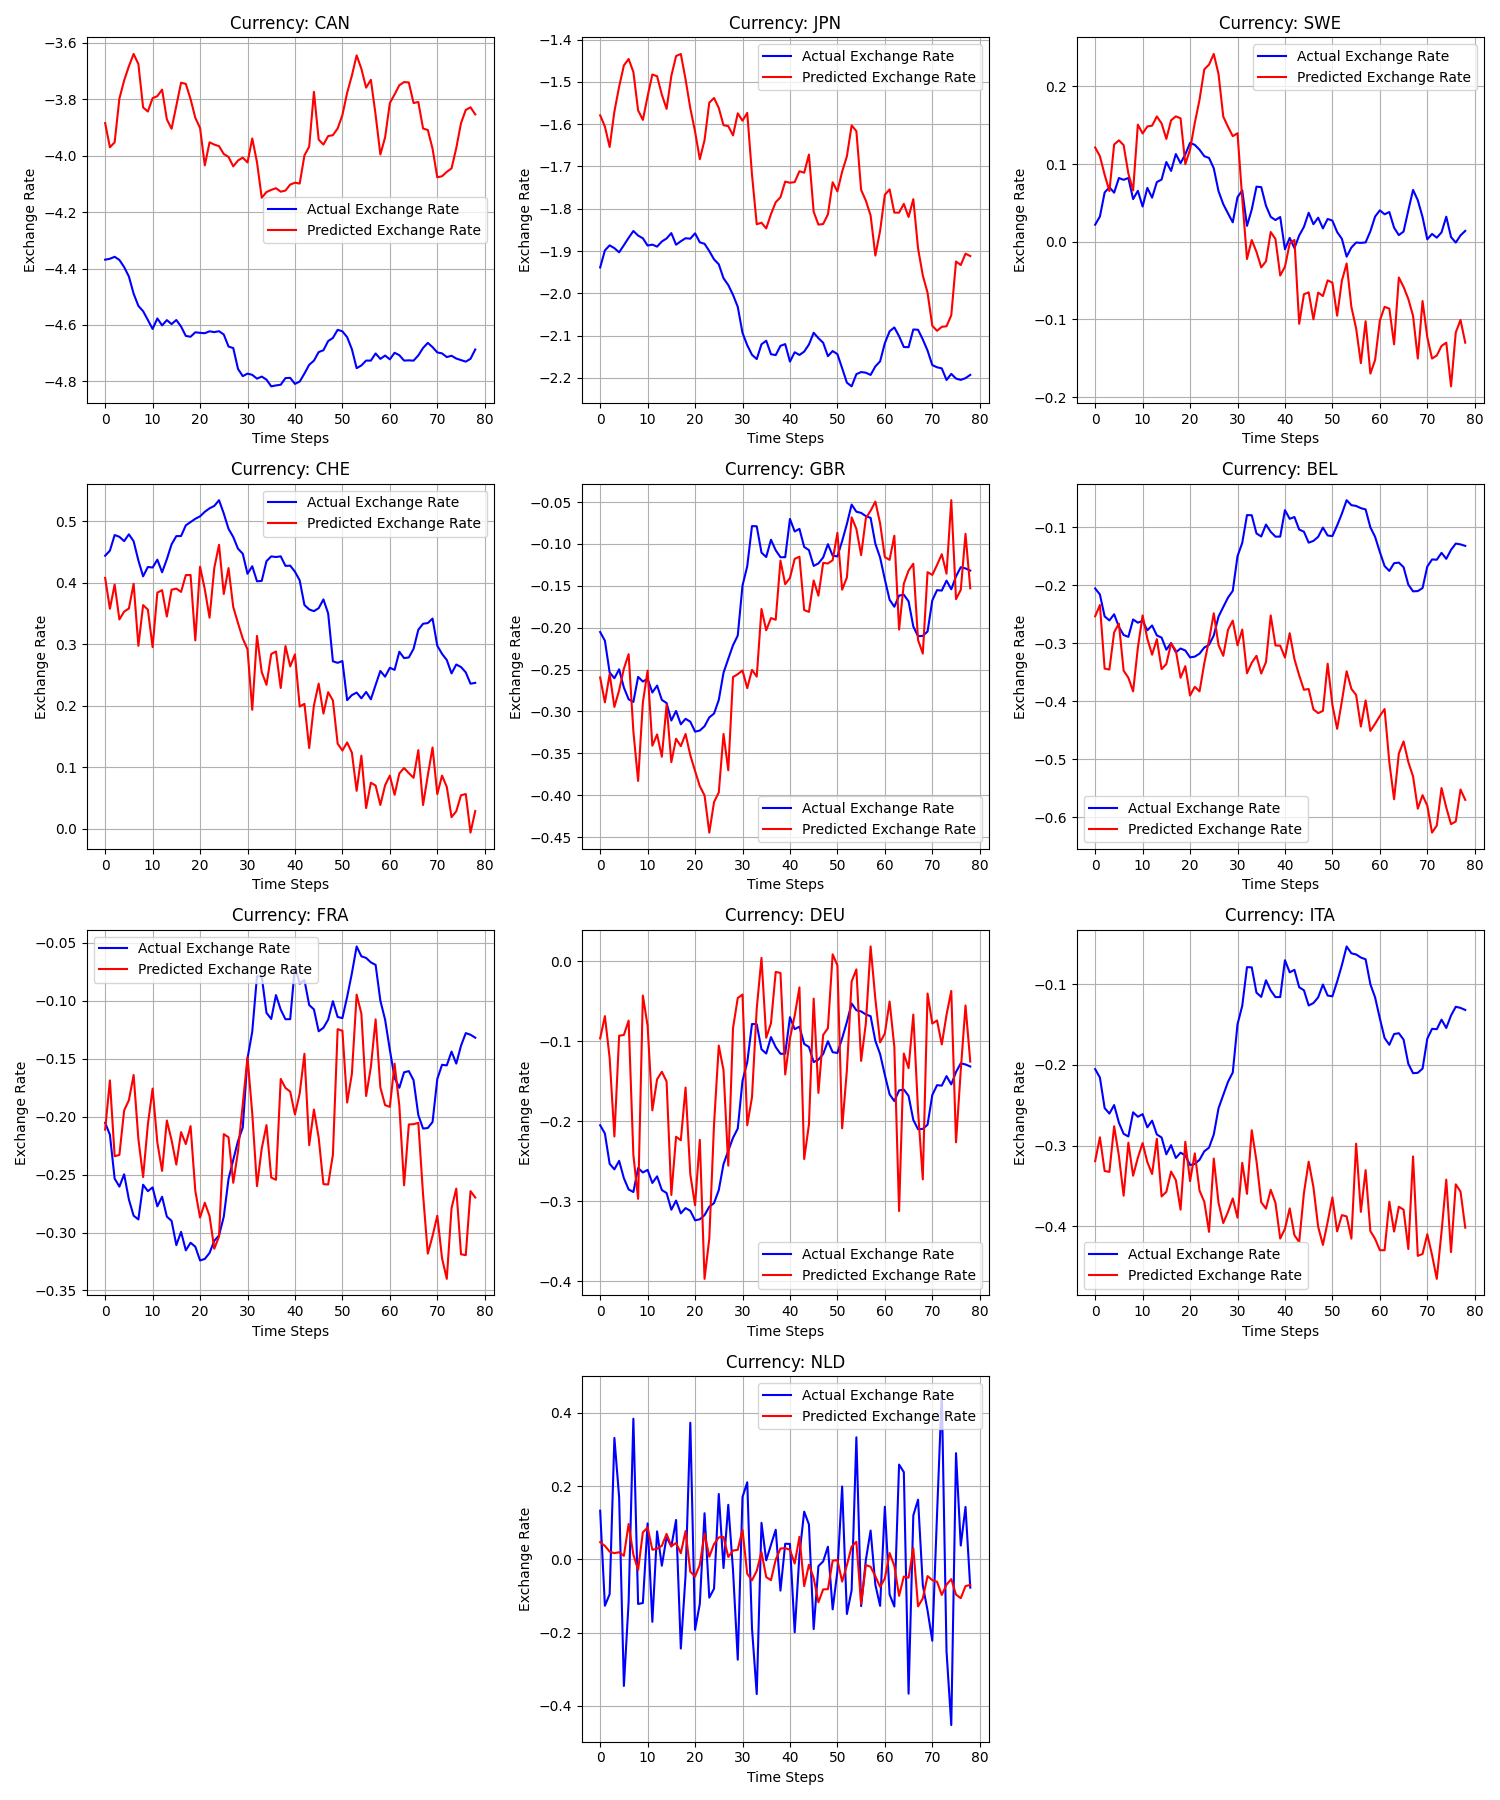
\includegraphics[width=0.8\textwidth]{figure/lstm_exchange_rate_predictions.png}
    \caption{LSTM Exchange Rate Predictions}
    \label{figure:lstm_predictions}
\end{figure}

\begin{figure}[ht]
    \centering
    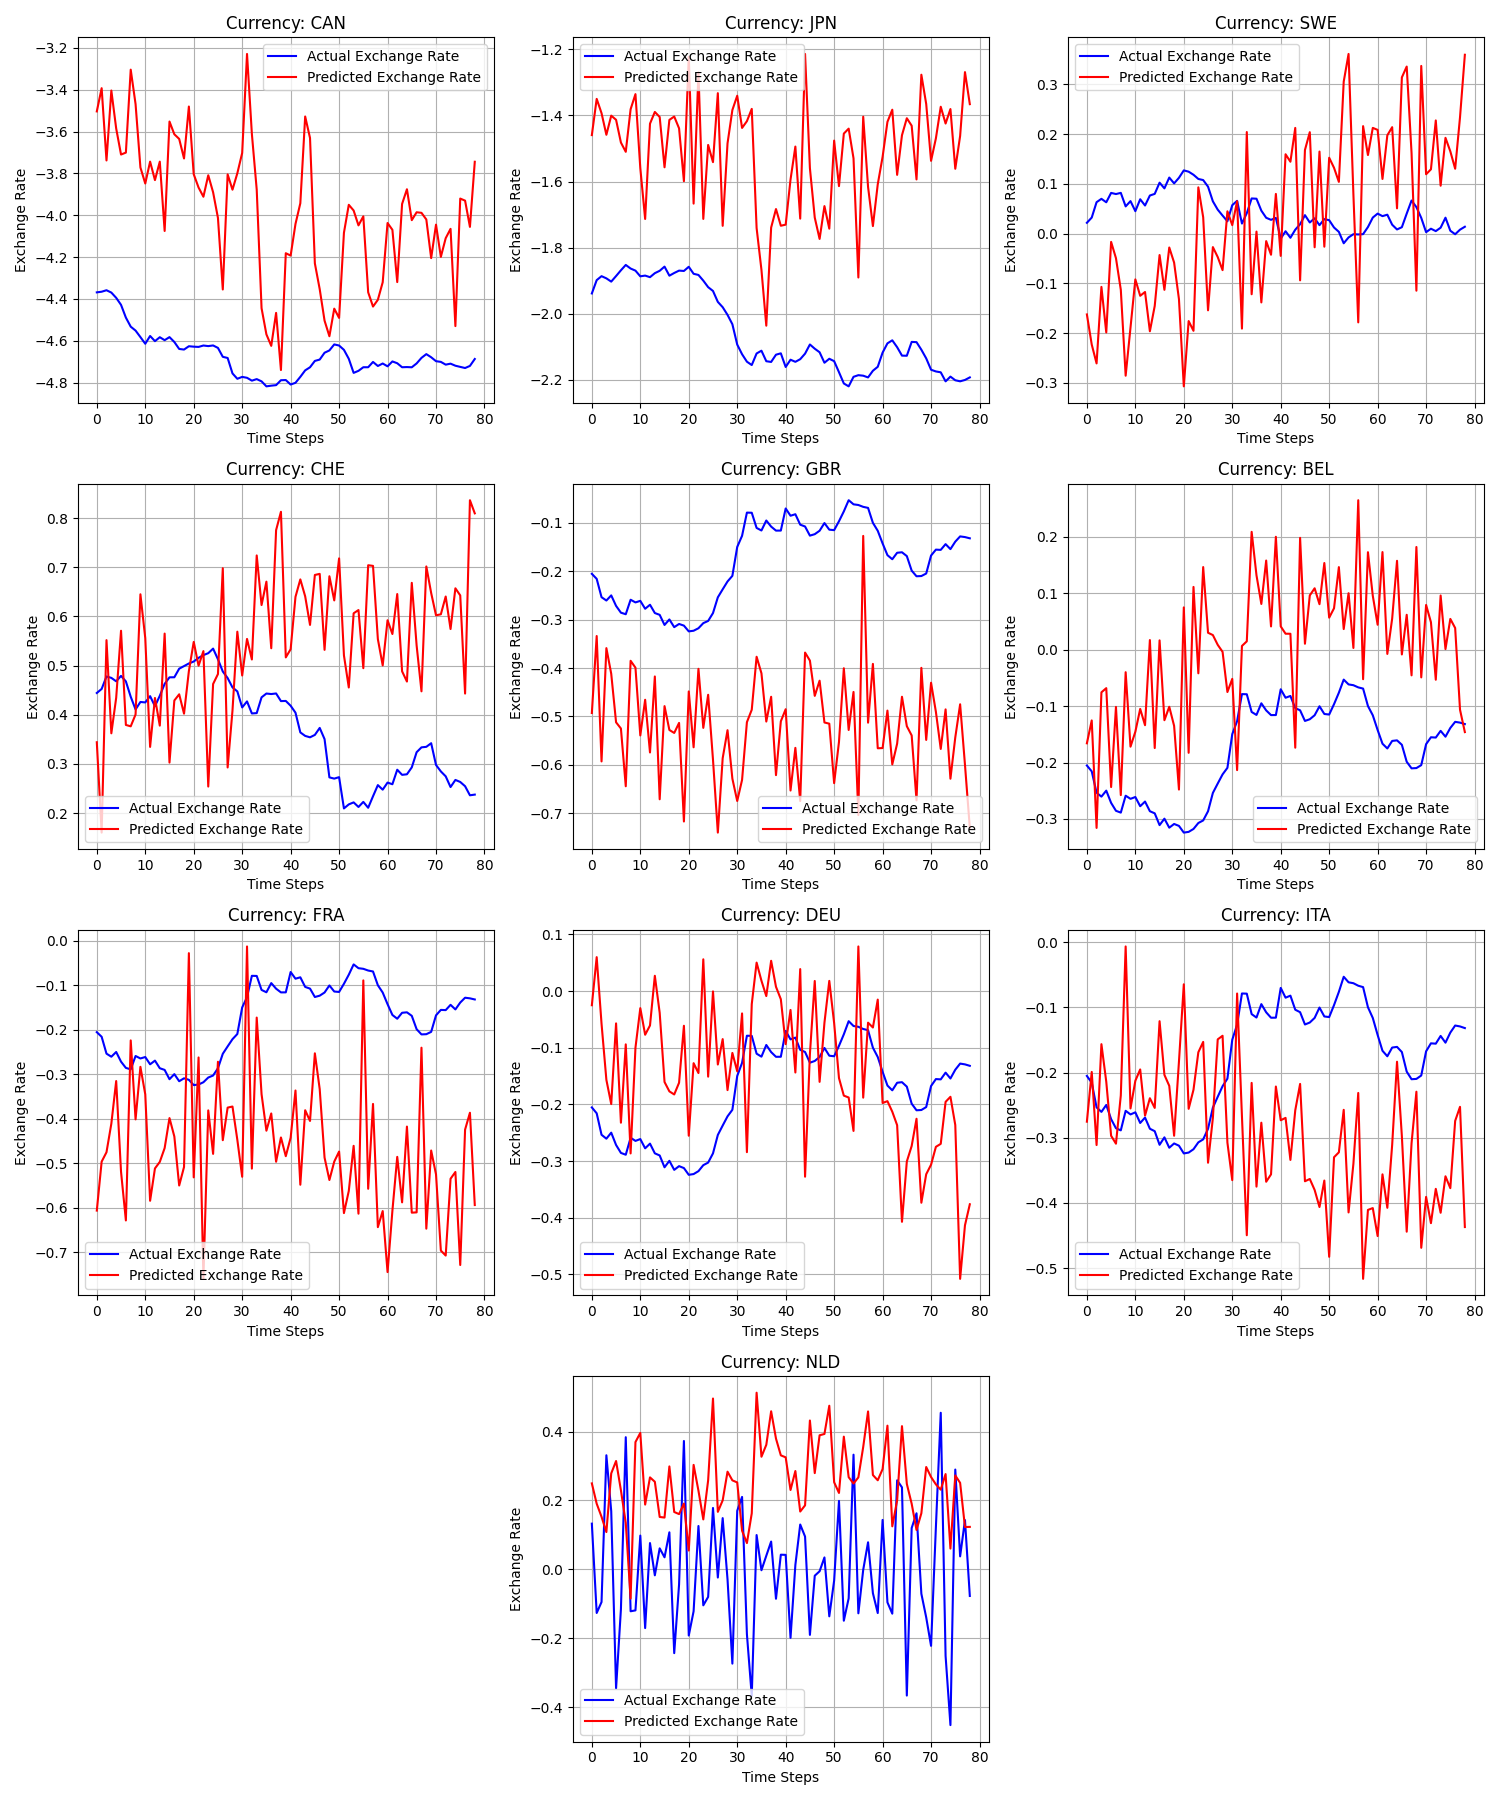
\includegraphics[width=0.8\textwidth]{figure/rnn_exchange_rate_predictions.png}
    \caption{RNN Exchange Rate Predictions}
    \label{figure:rnn_predictions}
\end{figure}

As observed in the figures, the LSTM model generally performed well in estimating the level and capturing the long-term trend of the time series and short-term changes. However, it struggled with sudden jumps, failing to predict these abrupt changes accurately. On the other hand, the RNN model exhibited challenges in capturing both the long-term trend and short-term fluctuations, with notable difficulties in predicting jumps.

\clearpage  % Ensure the figure and content appear on the same page

\subsection{Comparison on 1/N strategy}

Absolute returns are in percentages.

\subsubsection{Results for 2012-07-31 to 2015-12-31}

\begin{table}[h]
  \centering
  \csvautotabular{table/result_2012-07-31_2015-12-31.csv}
  \caption{Results for the period 2012-07-31 to 2015-12-31}
  \label{tab:results_2012-07-31_2015-12-31}
\end{table}

\subsubsection{Results for 2013-01-31 to 2016-12-31}

\begin{table}[h]
  \centering
  \csvautotabular{table/result_2013-01-31_2016-12-31.csv}
  \caption{Results for the period 2013-01-31 to 2016-12-31}
  \label{tab:results_2013-01-31_2016-12-31}
\end{table}

\subsubsection{Results for 2014-01-31 to 2017-12-31}

\begin{table}[h]
  \centering
  \csvautotabular{table/result_2014-01-31_2017-12-31.csv}
  \caption{Results for the period 2014-01-31 to 2017-12-31}
  \label{tab:results_2014-01-31_2017-12-31}
\end{table}

\clearpage  % Ensure the figure and content appear on the same page

\subsubsection{Results for 2015-01-31 to 2018-12-31}

\begin{table}[h]
  \centering
  \csvautotabular{table/result_2015-01-31_2018-12-31.csv}
  \caption{Results for the period 2015-01-31 to 2018-12-31}
  \label{tab:results_2015-01-31_2018-12-31}
\end{table}

\section{Analysis of the results}

The performance of all models across different periods shows consistently negative results in terms of log returns, absolute returns, and various performance metrics. The Sharpe ratios are particularly alarming, indicating significant underperformance compared to a risk-free rate. The Gain/Loss Ratio also suggests a lack of positive returns.

Possible reasons for such poor performance include inadequate model complexity, inappropriate parameter tuning, and the absence of crucial features in the input data. Since we performed cross-validation for ML-based data to fine-tune parameters more accurately, we may see that the reason is that we oversimplified the market model. If we were to include more market metrics and possibly some popular stock indices in the given country, it could have helped us assess the data better and develop a more sophisticated and better-performing model. 

The highly negative skewness and kurtosis values also highlight the models' struggle to capture extreme market events and sudden changes. The limitations in predicting jumps in machine learning and econometric models may also suggest that additional data could enhance the models' performance. Apart from the features used, such as 'Log-nominal exchange rate', 'Real Change to 12-M Average exchange rate', 'Inflation' and 'Interest Rate,' incorporating monthly realised volatility for each currency might have provided valuable information to help both RNN and LSTM models better capture abrupt changes in exchange rates.

Further investigation into incorporating additional relevant features might improve the models' ability to capture market dynamics and enhance overall performance.

\subsection{Delve deeper into TVECM dominance}

It is clear that despite not being that much better than the other models, TVECM is the best out of the worst. And while the provided data doesn't offer specific insights into why TVECM outperformed other models, we can make general observations based on the presented metrics. It's important to note that these are speculative explanations, and a more detailed analysis would require examining the model specifications, data characteristics, and additional information.

\textbf{Long-Term Dynamics:} TVECM (Time-Varying Error Correction Model) is designed to capture time-varying long-term relationships in a system. If the underlying market dynamics during the specified periods had significant time-varying components that TVECM could effectively model, it might have an advantage in predicting returns.

\textbf{Adaptability to Structural Changes:} TVECM is known for its ability to adapt to structural changes in the data. If there were fundamental shifts or changes in market behaviour during the analysed periods, TVECM might have been more effective in adjusting to these changes than VAR, LSTM, or RNN.

\textbf{Data Characteristics:} TVECM may perform well when dealing with cointegrated time series and capturing equilibrium relationships between variables. TVECM could leverage these relationships for better forecasting if the market data exhibited strong cointegration patterns.

\textbf{Parameter Sensitivity:} The performance of models like VAR, LSTM, and RNN heavily depends on parameter tuning. If these models were not correctly tuned for the specific characteristics of the financial data or the hyperparameters were not optimised, it could lead to suboptimal performance.

\textbf{Model Complexity:} TVECM might have balanced capturing complex relationships and avoiding overfitting. In situations where simpler models outperform more complex ones due to limited data or noise, TVECM's relatively more uncomplicated structure could have been an advantage.

\subsection{Comparison with Wang}

In examining the performance of the LSTM model relative to TVECM, RNN, and VAR, several noteworthy trends emerge. 

\subsubsection{LSTM vs. TVECM}

Contrary to the findings in Wang et al.'s study, our analysis indicates that TVECM outperformed LSTM across the considered time periods. This discrepancy may arise from differences in model specifications, data characteristics, or specific economic conditions prevailing during the analysed periods.

\subsubsection{Consistent Superiority over RNN and VAR}

While LSTM did not outperform TVECM, it demonstrated consistent superiority over RNN and VAR. This aligns with broader trends observed in Wang et al.'s study, where LSTM tended to outperform simpler models such as RNN and VAR.

\subsubsection{Performance Dynamics Over Time}

A crucial aspect of the analysis involves examining how LSTM's performance varied over different time periods. Interestingly, LSTM performed better than TVECM as we proceeded further away from the data on which our model was trained. Since all the models performed generally severely, this may only imply that TVECM degenerates faster than LSTM.

\subsubsection{Realised Returns at the Currency Pair Level}

Although the provided data lacks specific information on realised returns at the currency pair level, exploring this aspect could offer deeper insights into the factors influencing LSTM's performance, especially when models suggest conflicting strategies.

\section{Conclusion}

This paper contributes to the literature by introducing LSTM networks to predict carry trade returns. LSTM networks, initially developed by Hochreiter and Schmidhuber (1997), have the unique ability to memorise long-term data patterns, optimising explanatory factors and data length. The analysis is conducted on a monthly dataset spanning G10 currencies between 1990 and 2019, revealing that LSTM networks underperformed traditional models regarding average return, Sharpe ratio, and gain/loss ratio, which is different from Wang et al. findings.

The findings of this paper indicate a deterioration in carry trade returns after the 2007–2008 global financial crisis, consistent with the trend observed in interest rate differentials shrinking to near zero \cite{accominotti2019currency}, and in our case to even negative long-term returns. This provides supportive evidence that excess carry trade returns may be influenced by long-term changes in interest rate differentials, aligning with the UIP hypothesis.

The observed underperformance of LSTM during the 2015-2018 period prompts a closer look at long-term trends, potential structural changes, and shifts in market dynamics during that specific timeframe. However, this includes deep macroeconomic analysis, the exploration of the applicability of LSTM networks in other economic settings, and further investigating the nuanced features of carry trade returns, especially in the context of evolving market conditions post-financial crisis, which may be a sound basis for future research.

% Specify the bibliography style and file
\bibliographystyle{unsrt}
\bibliography{references}

\appendix

\section{ML Foundations}

\subsection{Long Short-Term Memory (LSTM)}\label{appx:lstm}

Long Short-Term Memory (LSTM) is an example of a recurrent neural network (\hyperref[appx:rnn]{RNN}) architecture designed to overcome the vanishing gradient problem associated with traditional RNNs. LSTMs are particularly well-suited for sequence prediction tasks, making them popular in various fields, including time series forecasting and natural language processing.

LSTMs incorporate memory cells and gating mechanisms, allowing them to capture long-term dependencies in sequential data. The fundamental components of an LSTM include the input gate, forget gate, memory cell, and output gate. These gates regulate the flow of information within the LSTM, enabling it to retain or discard information over time selectively.

The information flow within an LSTM can be outlined as follows:

\begin{enumerate}
  \item \textbf{Forget Gate:} Determines how much of the previous cell state should be retained and how much should be forgotten.

  \item \textbf{Input Gate:} Controls the amount of new information that should be added to the cell state.

  \item \textbf{Memory Cell:} Stores and updates information based on the input and previous cell state.

  \item \textbf{Output Gate:} Determines the next hidden state based on the current input and cell state.

\end{enumerate}

Figure \ref{figure:lstm_structure} illustrates an LSTM network's structure, showcasing the information flow through the gates and the memory cell.

\begin{figure}[ht]
  \centering
  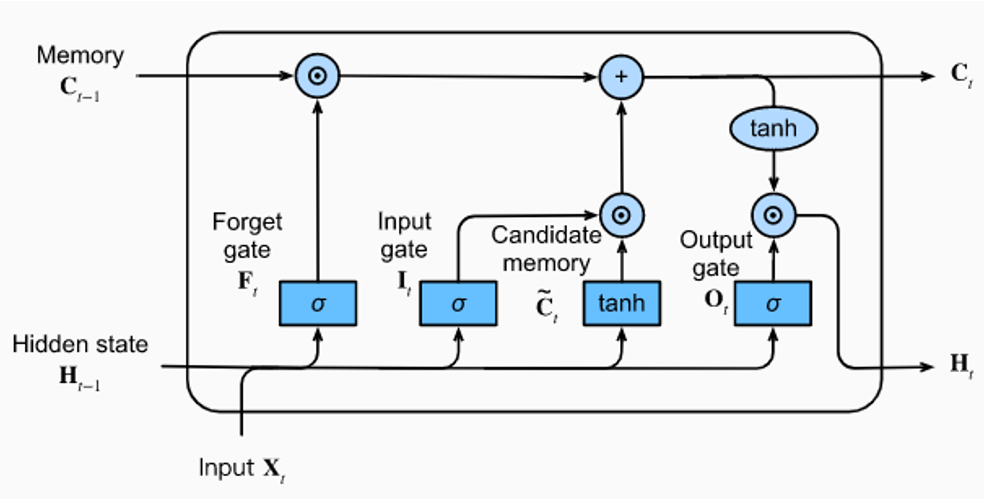
\includegraphics[width=0.8\textwidth]{figure/lstm.png}
  \caption{Structure of a Long Short-Term Memory (LSTM) Network}
  \label{figure:lstm_structure}
\end{figure}

LSTMs have demonstrated superior performance in capturing complex patterns and dependencies in sequential data, making them valuable in various machine-learning applications.

% \clearpage  % Ensure the figure and content appear on the same page

\subsection{Recurrent Neural Network (RNN)}\label{appx:rnn}

Recurrent Neural Networks (RNNs) are designed for sequential data processing and capture dependencies and patterns across time. They have connections that form directed cycles, allowing them to maintain a hidden state that stores information about previous inputs. However, traditional RNNs suffer from the vanishing gradient problem, which limits their ability to capture long-term dependencies. More advanced architectures like Long Short-Term Memory (\hyperref[appx:lstm]{LSTM}) networks have been developed to overcome this limitation.

\section{Economic Foundations}

\subsection{Efficient Market Hypothesis (EMH)}\label{appx:emh}

The Efficient Market Hypothesis (EMH) is a fundamental concept in financial economics that posits that financial markets efficiently incorporate and reflect all relevant information. According to EMH, it is not possible for an investor to consistently achieve higher-than-average returns through the analysis of historical price movements or publicly available information. The hypothesis suggests that asset prices fully reflect all available information, making it impossible to achieve consistent profits by exploiting market inefficiencies.

EMH is typically categorized into three forms:

\begin{enumerate}
  \item \textbf{Weak Form EMH:} Assumes that past price and volume information is already incorporated into current stock prices. Therefore, technical analysis relying on historical price movements would not provide an advantage.

  \item \textbf{Semi-Strong Form EMH:} Posits that all publicly available information is already reflected in stock prices. Consequently, neither fundamental analysis (examining financial statements) nor technical analysis can consistently outperform the market.

  \item \textbf{Strong Form EMH:} Asserts that all public or private information is fully reflected in asset prices. This implies that even insider information cannot be used to achieve superior returns consistently.
\end{enumerate}

EMH has important implications for investors, as it challenges the effectiveness of active trading strategies and supports the notion that a passive buy-and-hold approach may be just as practical in the long run.

\subsection{Uncovered Interest Parity (UIP)}\label{appx:uip}

Uncovered Interest Parity (UIP) is an economic theory in international finance that explores the relationship between interest rates and exchange rates. UIP posits that the expected change in the exchange rate between two currencies is equal to the difference in their nominal interest rates. In other words, when investors do not hedge their currency exposure, they should expect to earn the same return on investment in any currency, regardless of the level of interest rates.

Mathematically, UIP can be expressed as: $ \mathbf{E}(e_{t+1}) = i_t - i^*_t $, where \( \mathbf{E}(e_{t+1}) \) is the expected change in the exchange, \( i_t \) is the domestic interest rate and \( i^*_t \) is the foreign interest rate.

If UIP holds, investors should not be able to profit consistently from differences in interest rates across currencies. However, empirical studies have shown mixed evidence regarding the validity of UIP, with various factors influencing the observed relationship between interest rates and exchange rates.

\subsection{VAR model}\label{appx:var}

The VAR model extends a classical univariate model to a multivariate case by framing the considered set of variables into vectors. Following the original paper, the VAR with lag equal to 1 and the respective variable vector $y_t = [\Delta e_t, \pi^{*}_t - \pi_t, i^{*}_t - i_t, q_t - \bar{q}]^t$ has the following specification:

\begin{equation}
    y_t = Ay_{t-1} + \epsilon_t
\end{equation}

where A is a time-invariant ($4 \times 4$) coefficients matrix, $\epsilon_t$ - zero-mean i.i.d. ($4 \times 1$) error vector with a fixed covariance matrix. 

Note that this specification is vulnerable to the autocorrelatedness of the variables. Thus, the estimation can only be performed on the differenced series, as in our case. The series is also assumed to be stationary. The coefficient matrix captures the cross relationships between the variables through the off-diagonal terms.

\subsection{TVECM}\label{appx:tvecm}

TVECM is an extension of the error correction version of the VAR model. Before addressing the threshold VECM, we describe the classical VECM. 

Keeping our vector of variables $y_t$, the vector autoregressive model with error correction term (VECM) and lag equal 1 has the following specification:

\begin{equation}
\Delta y_t = \Pi y_{t-1} + \Gamma\Delta y_{t-1} + \epsilon_t 
\end{equation}

where $\epsilon_t$ are zero-mean, independent error terms. The model assumes that each series is integrated of order one, i.e. $y_{it}$ ~ $I(1), i = 1, ... , 4$. Under this assumption of cointegration, we can find a stationary linear combination of  $y_{it}$, i.e. $\beta^t y_{it}$ ~ $I(0)$. Thus (2) can be rewritten according as 

\begin{equation}
\Delta y_t = \alpha\beta^ty_{t-1} + \Gamma\Delta y_{t-1} + \epsilon_t 
\end{equation}

where $\beta$ is a $1 \times 4$ vector of cointegration vector and $\alpha$ is a $4 \times 1$ loading vector. The impact of lagged values of $X_{it}$ are characterised by $\Gamma_i$, $i = 1,...,k$ $4 \times 4$ matrix. Note that here, we follow the suggestion of the original paper that assumes a unique cointegrating relationship with $q_t - \bar{q}$ being the cointegrating variable. Thus, the $\beta$ and $\alpha$ are treated as vectors, even though generally, they represent matrices with size dependent on the number of cointegrating relationships. 

In essence, VECM is a model that implies the existence of a long-run stationary relationship between the variables determined by the cointegrating vector while at the same time allowing for short-run deviations from the stationary path described by the $\Gamma$ matrix. The threshold version of VECM assumes multiple stationary regimes for the same stationary long-run path, thus allowing for non-linear long-run relation modelling. We follow the original paper methodology, assuming the presence of 2 regimes. 

\end{document}
